\begin{figure}[h]
\centering
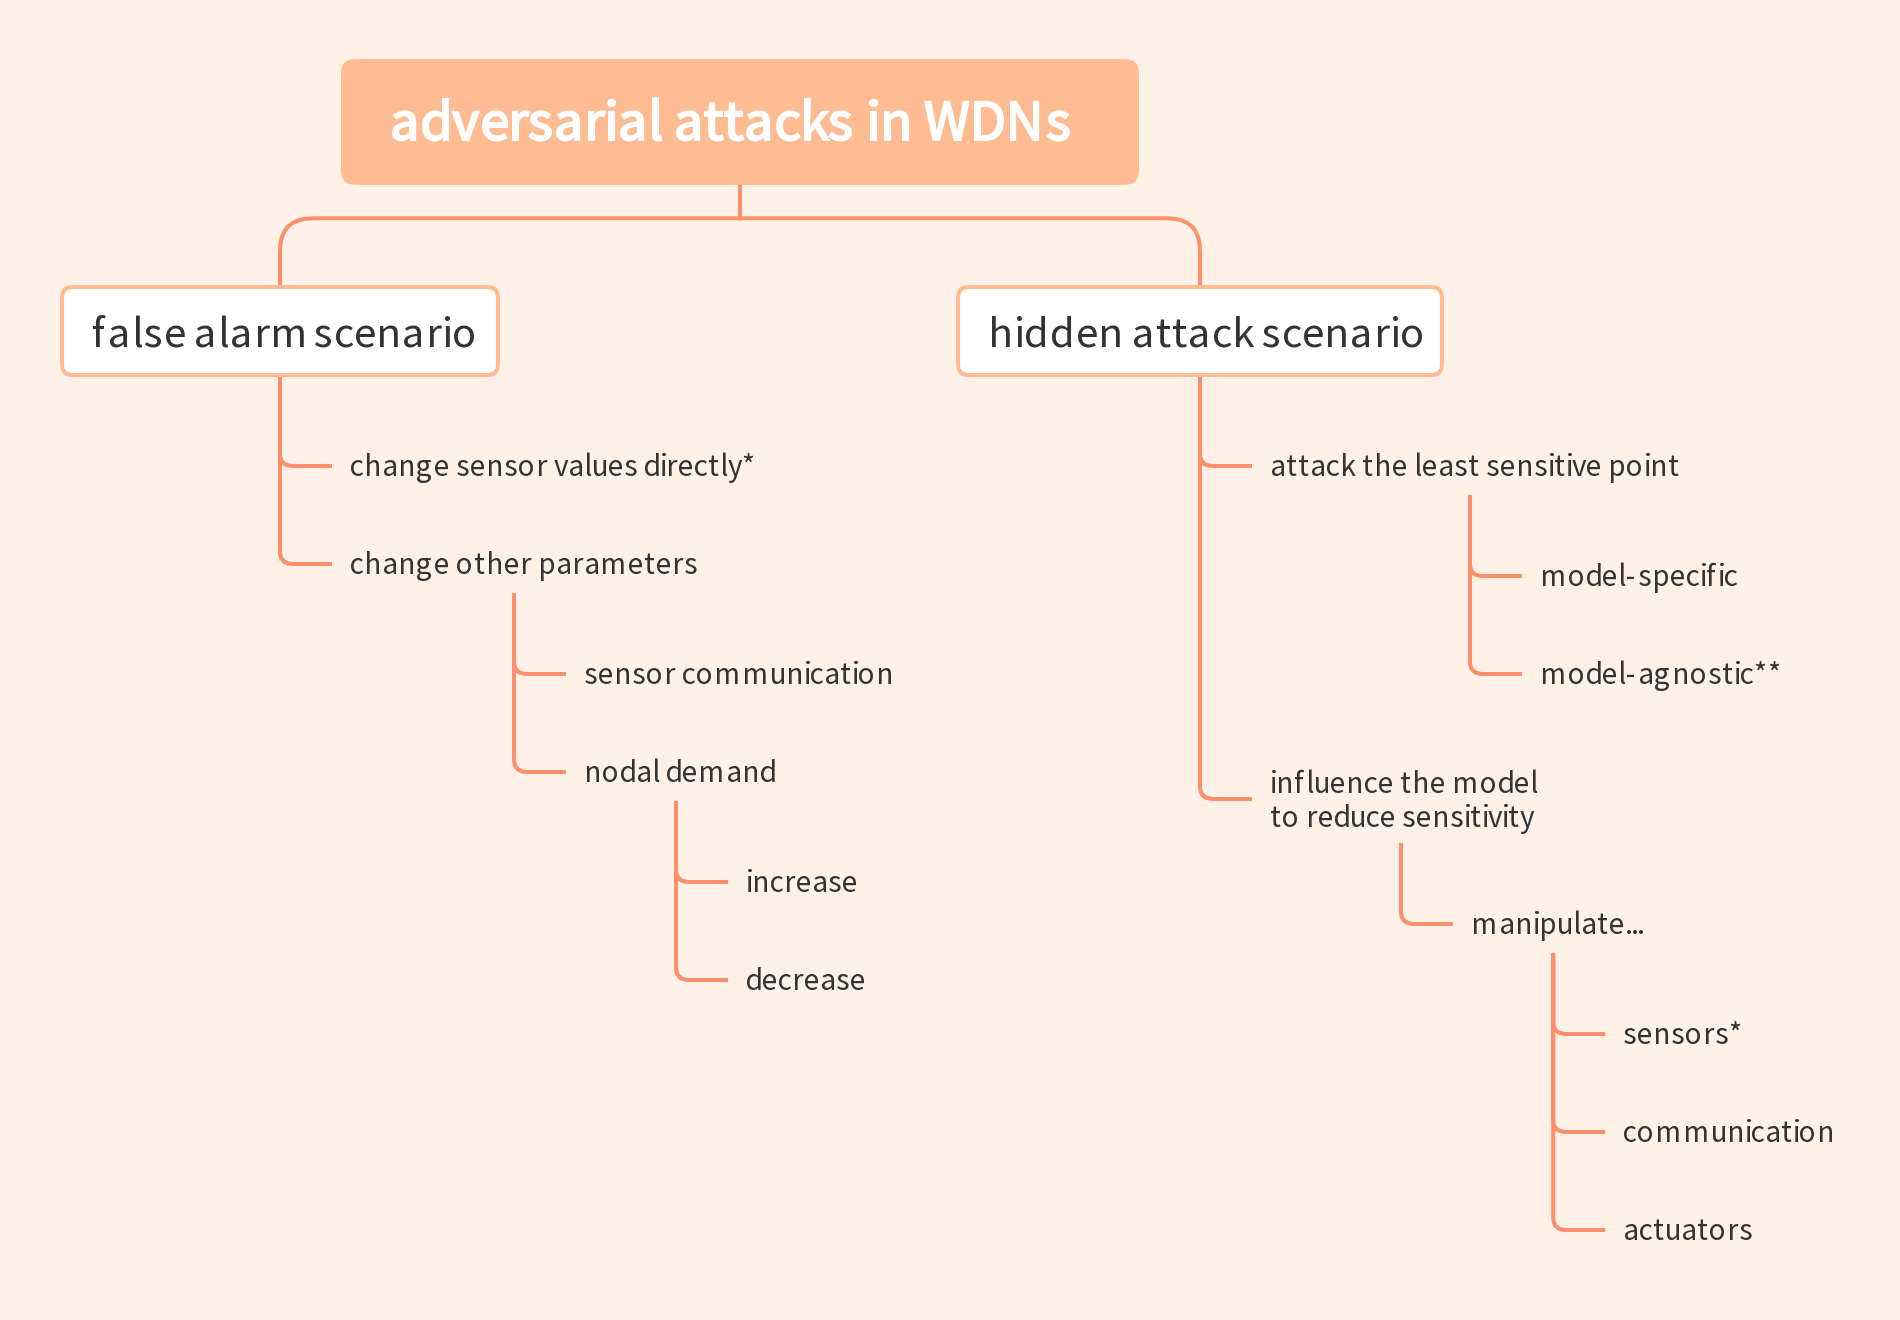
\includegraphics[height=\textheight,width=\textwidth,keepaspectratio=true]{Figures/adversarials_in_WDNs.png}
\caption{Taxonomy showing different types of adversarial attacks in WDNs
\newline * Methods proposed in \cite{conaml}
\newline ** Metholds proposed here}
\label{fig:adversarial_taxonomy}
\end{figure}

There exist two different scenarios how a detector could be fooled:
The first one would be an input causing the
detector to predict a leak, even though no leak is actually present.  We refer
to this as the false alarm scenario;
The second one would be an input causing
the detector not to predict a leak, even though there is one.  This case can
be termed the hidden attack scenario. 

In case of the false alarm scenario, there are again two different
possibilities of attacking the system: An adversary might try to manipulate a
few network elements (e.g. sensors, pipes, etc.) they have managed to access or the attacker makes
external changes to the water demand at certain nodes.  Note that, even if the
adversary has managed to gain control over some parts of the network
infrastructure, they are not interested in actually creating a leak or other
damage in this scenario, but rather aims at causing the leakage detector to
raise a false alarm. Thus, manipulating sensor values or disturbing the
inter-sensor communication might be a promising approach. In particular, a
large decrement of pressure measurements or the complete abortion of sensory
recordings are likely to cause a wrong leakage prediction. In the attack scenario where the attacker can change node demands only, the success of the attack will depend on the number of nodes under
adversary control and the extent to which the demand can be changed at these
nodes. Generally, both a high increase in the demand e.g. by opening all water
taps in an industrial complex as well as a high decrease constitute possible
reasons for a prediction failure resulting in a false alarm.

The hidden attack scenario always involves an adversary who creates an actual
leak in the physical network. In order to fool the leakage detector
 not to find the leak, there are again two possibilities: The attacker could
try to manipulate the detector in order to make it less sensitive or they
could place the leak at a point where the detector is not very sensitive
anyway.  In the manipulation case, sensors, programmable logic controllers
(PLCs) or the sensory control and data acquisition system (SCADA) could be
targets of the attack\footnote{These constituents of a network monitoring
system were used in the Battle of the Attack Detection Algorithms (BATADAL)
\cite{batadal}. A monitoring system might have additional entry points for an
attack in practise.}. Otherwise, the adversary will have to search for points
in the network where the detector has little sensitivity to leaks.

Because investigating all the aforementioned attack scenarios in detail is behind the scope of this work, we focus on a particular type of hidden attack: Searching for locations in the network where the detector is the least sensitive to leaks.
